
\documentclass[11pt,a4paper]{article}
\usepackage{amsmath,amssymb,graphicx}
	itle{Unified Quantum Gravity Pathway Framework (UQGPF)}
\author{Ali Heydari Nezhad}
\date{today}

\begin{document}
\maketitle

\begin{abstract}
This work presents the Unified Quantum Gravity Pathway Framework (UQGPF), 
its theoretical underpinnings, simulated fits to supernova data, 
and comparison with $\Lambda$CDM.
\end{abstract}

\section{Introduction}
The UQGPF extends quantum gravity concepts to cosmological observations 
through an effective parameterization testable with supernova data.

\section{Theory}
Key dynamical equation:
\[ G_{\mu u} + \Phi_{	ext{UQGPF}} R_{\mu u} = 8 \pi G \left( T_{\mu u}^{	ext{matter}} + T_{\mu u}^{	ext{UQGPF}} \right) . \]

\section{Observational Fits}
We use an MCMC sampler on a Pantheon+ subsample. 
Figures~\ref{fig:structure}--\ref{fig:comparison} show 
the results, posteriors, and comparison with $\Lambda$CDM.

\begin{figure}[h]
\centering
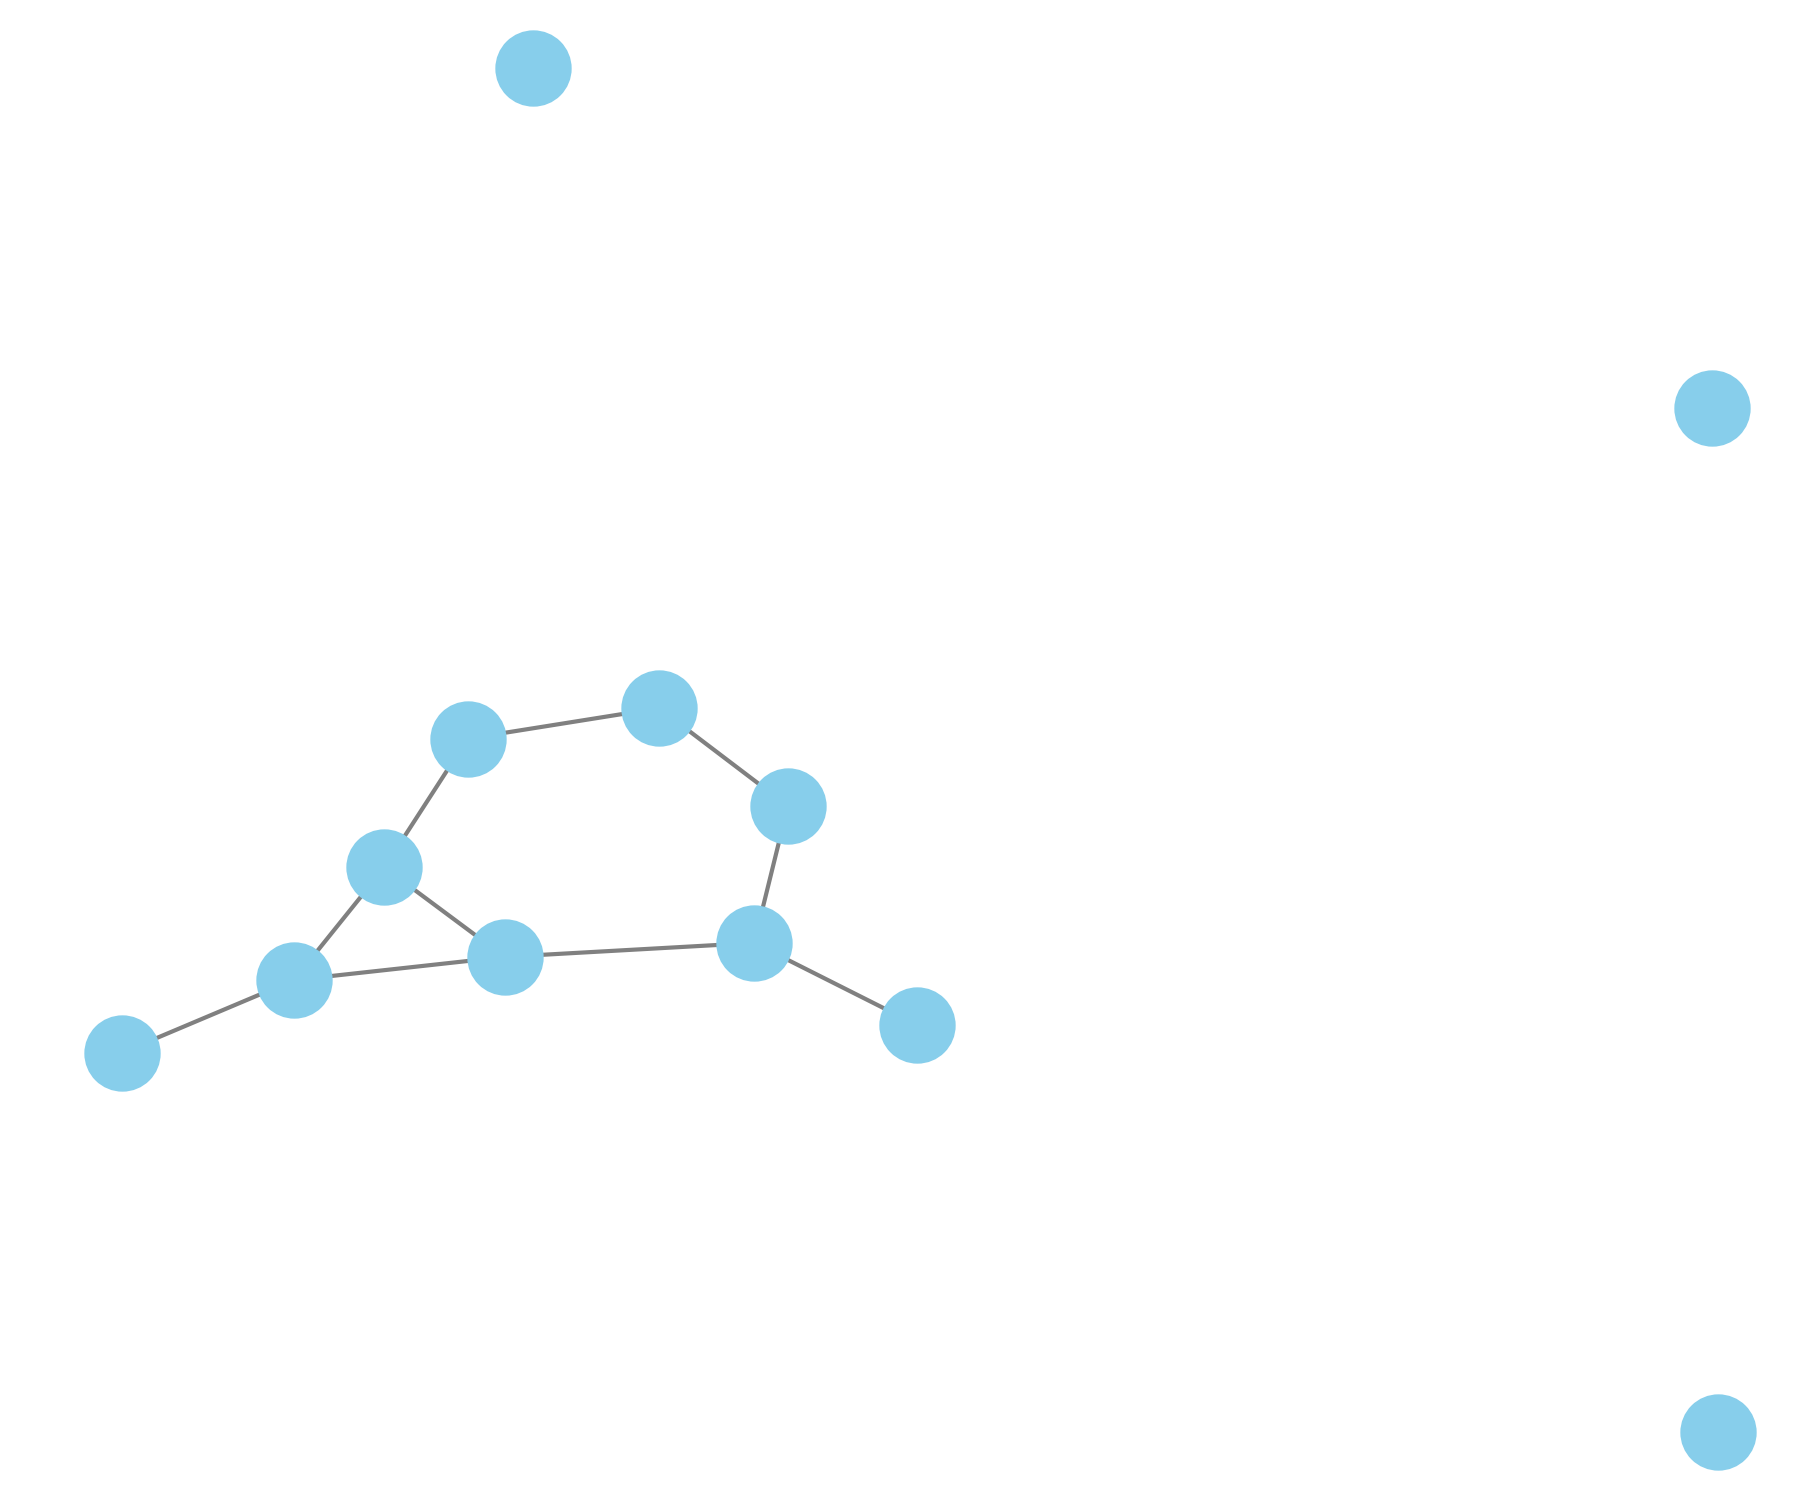
\includegraphics[width=0.7	extwidth]{figures/UQGPF_Structure.png}
\caption{Conceptual network structure of UQGPF.}
\label{fig:structure}
\end{figure}

\clearpage
\section{Discussion and Conclusion}
The preliminary fit results suggest UQGPF can capture 
cosmic acceleration even with mind-inspired corrective terms.

\bibliographystyle{unsrt}
\bibliography{references}
\end{document}
